\documentclass[
  11pt,
  fleqn
]{article}
% [fleqn] left-aligns all equations

% fonts

\usepackage[T1]{fontenc} % Apparently this
% https://tex.stackexchange.com/questions/287312/font-not-loadable-metric-data-not-found-or-bad
\usepackage[full]{textcomp}
\usepackage[final,expansion=alltext,nopatch=footnote]{microtype}
\usepackage{csquotes} % suppress warning from `babel`
\usepackage[english]{babel}
\usepackage[fleqn]{mathtools}
\usepackage[cal=boondoxo]{mathalpha} % mathcal

\usepackage{amsthm} % gives proof environment:
% https://www.overleaf.com/learn/latex/Theorems_and_proofs

\usepackage{newtxtext}
% \usepackage{txfonts} % See
% https://tex.stackexchange.com/questions/444243/symbols-not-showing-up

% These need to be after newtxtext
\usepackage[varqu,varl]{inconsolata} % sans serif typewriter
% \usepackage{cabin} % sans serif - ugly

\usepackage[bigdelims,vvarbb]{newtxmath} % bb from STIX % "should be
% loaded AFTER the text font" -
% https://mirrors.mit.edu/CTAN/fonts/newtx/doc/newtxdoc.pdf

% geometry of the page

\usepackage[
  % top=1in,
  % bottom=1in,
  % left=1in,
  % right=1in
]{geometry}

% paragraph spacing

\setlength{\parindent}{0pt}
\setlength{\parskip}{1.5ex plus 0.4ex minus 0.2ex}

% useful packages

% \usepackage{natbib} % incompatible with BibLaTeX
\usepackage{epsfig}
\usepackage{url}
\usepackage{bm}
\usepackage{blindtext}

% Leon additions

\usepackage{enumitem} % allows for enumerate[resume]

\usepackage{booktabs}

\usepackage[
  style=authoryear-comp,
  natbib=true,
  % refsection=chapter,
  url=false,
  doi=true,
  isbn=false,
  date=year %
  % https://tex.stackexchange.com/questions/55780/disable-month-in-biblatex-bibliography
]{biblatex} % natbib=true allows \citep
% Clear "visited on"
% https://tex.stackexchange.com/questions/400384/how-to-disable-biblatex-showing-visited-on-on-the-references
\AtEveryBibitem{
  \clearfield{urlyear}
  \clearfield{urlmonth}
  \clearfield{eprint} % remove PMID %
  % https://tex.stackexchange.com/questions/250784/removing-eprint-and-eprinttype-in-citation-notes
}

\usepackage{graphicx}
% ensures figures stay in their section
% https://tex.stackexchange.com/questions/279/how-do-i-ensure-that-figures-appear-in-the-section-theyre-associated-with
\usepackage[section]{placeins}

% Section formatting using titlesec
\usepackage{titlesec}
\titleformat*{\section}{\singlespacing\sffamily\Large}
\titleformat*{\subsection}{\singlespacing\sffamily\large}
% \titleformat*{\subsubsection}{\itshape}
\titleformat*{\paragraph}{\itshape}
\titleformat{\chapter}{\singlespacing\sffamily\Huge}{{\thechapter}}{1em}{}

% center figures by default
\makeatletter
\g@addto@macro\@floatboxreset\centering
\makeatother
% italic figure captions
\usepackage[format=plain,
  textfont=it,
]{caption}

% simple TO DO and comment macros
\usepackage[
  % https://tex.stackexchange.com/questions/4503/how-do-i-specify-color-in-rgb-using-hypersetup-in-hyperref
  dvipsnames,svgnames,x11names
]{xcolor}
\newcommand\todo[1]{\textcolor{orange}{[#1]}}% simple TO DO macro
\newcommand\comment[1]{\textcolor{red}{[#1]}}

\usepackage{url}
\usepackage[
  hidelinks,
  pdfa % Required for valid pdf/a output:
  % https://tex.stackexchange.com/questions/431022/pdf-a-validation-problem-the-f-key-is-missing
]{hyperref}
\hypersetup{
  % colorlinks,
  % linkcolor=RoyalBlue4,
  % citecolor=PaleVioletRed4,
  % urlcolor=Firebrick4
}

\newcommand{\indsim}{\overset{\mathrm{ind}}{\sim}}
% https://tex.stackexchange.com/questions/60545/should-i-mathrm-the-d-in-my-integrals
\newcommand*\diff{\mathop{}\!\mathrm{d}}
\newcommand*\Diff[1]{\mathop{}\!\mathrm{d^#1}}
\newcommand{\e}{\mathrm{e}}
\newcommand{\E}{\mathrm{E}}
\renewcommand{\P}{\mathrm{P}}
\newcommand{\N}{\mathrm{N}}
\newcommand{\diag}{\mathrm{diag}}
\newcommand{\ave}{\mathrm{ave}}
\newcommand{\Var}{\mathrm{Var}}
\newcommand{\Cov}{\mathrm{Cov}}
\newcommand{\cov}{\mathrm{cov}}
\newcommand{\sd}{\mathrm{sd}}
\newcommand{\var}{\mathrm{var}}
\newcommand{\corr}{\mathrm{corr}}
\renewcommand\vec{\boldsymbol}

% Overlap-specific
\newcommand{\rank}{R}
\newcommand{\rmax}{m}
\newcommand{\rgap}{r^\text{gap}}
\newcommand{\Ngap}{N_1^\text{gap}}
\newcommand{\pigap}{\pi_1^\text{gap}}

% For appearance of block matrices
% https://tex.stackexchange.com/questions/495903/horizontal-and-vertical-lines-in-pmatrix
\renewcommand{\arraystretch}{1.5}

% Theorem-type environments
\newtheorem{definition}{Definition}[section]
\newtheorem{result}[definition]{Result}
\newtheorem{claim}[definition]{Claim}

% From Datta template
% https://github.com/bibekanandadatta/JHU-Dissertation-Template

\usepackage{setspace}                         % sets space between lines

%%%% JH Library requirement (DO NOT CHANGE)
\def\GlobalMargin{1.0in}                      % margin on all sides
% \def\PrintingOffset{0.5in}                  % additional left
% margin for the printed copy
\def\PrintingOffset{0.0in}
\def\MainTextSpacing{\singlespacing}        % double-spaced main text
% \def\MainTextSpacing{}
\def\CaptionStretch{1.1}                    % to match 2x spacing
% \def\CaptionStretch{1.0}

\captionsetup{font={stretch=\CaptionStretch}}

\geometry{
  letterpaper,
  margin=\GlobalMargin,
  bindingoffset=\PrintingOffset,
  nomarginpar,
  % includehead,
  % headheight=\HeaderHeight,
  % headsep=\HeaderSpace,
  includefoot,
  heightrounded
}

%%%% BIBLIOGRAPHY ITEMS
\def\BibTextSpacing{\onehalfspacing}         % single-spaced bibliography
% \def\BibTextSpacing{\singlespacing}         % single-spaced bibliography
\def\BibItemSpacing{\baselineskip}          % spacing between
% bibliographic items in reference

%%%% UNNUMBERED CHAPTERS, SECTION, and SUBSECTION COMMAND for ADDING to TOC
%% removes the 'Chapter #' title while keeping it listed in the TOC
\newcommand\chap[1]{%
  \chapter*{#1}%
  \markboth{#1}{}
\addcontentsline{toc}{chapter}{#1}}

%% removes the 'Section #' title while keeping it listed in the TOC
\newcommand\sect[1]{%
  \phantomsection
  \section*{#1}%
\addcontentsline{toc}{section}{#1}}

%% removes the 'Subsection #' title while keeping it listed in the TOC
\newcommand\subsect[1]{%
  \phantomsection
  \subsection*{#1}%
\addcontentsline{toc}{subsection}{#1}}

%% removes the 'Subsubsection #' title while keeping it listed in the TOC
\newcommand\subsubsect[1]{%
  \phantomsection
  \subsubsection*{#1}%
\addcontentsline{toc}{subsubsection}{#1}}

% Correct matrix for double spacing
% https://tex.stackexchange.com/questions/137004/matrix-within-equation/137009#137009
\makeatletter
\def\env@matrix{\hskip -\arraycolsep
  \let\@ifnextchar\new@ifnextchar
  \linespread{1}\selectfont
  \renewcommand{\arraystretch}{1.2}%
\array{*\c@MaxMatrixCols c}}
\makeatother

% Footnotes must be 2 points less than main text but larger than 8pt
\usepackage{footmisc}
\renewcommand{\footnotesize}{\fontsize{9pt}{11pt}\selectfont}

% For including CV
\usepackage{pdfpages}

% Generate PDF/A (archival format)
% https://webpages.tuni.fi/latex/pdfa-guide.pdf
\usepackage[a-1b,mathxmp]{pdfx}

\usepackage[
  nottoc % Don't include TOC in TOC
]{tocbibind}

% Redefine `abstract`s so they can be at the start of each chapter
% don't cause the page numbering to reset
% https://tex.stackexchange.com/a/4857
\newenvironment{myAbstract}{
  \rightskip.5in
  \leftskip.5in
  % \itshape
}{}

% For writing/planning purposes: show paragraph level in TOC
\setcounter{secnumdepth}{3}

\addbibresource{references.bib}
\graphicspath{{fig/}}

\title{Constructing ordinal outcomes for clinical trials}
\author{Leon Di Stefano + Ordinal
Working Group}
\date{\today}

\begin{document}

\maketitle

\begin{abstract}
  Ordinal outcomes or endpoints are an increasingly popular choice in
  clinical trials.
  They have been recently popular in the study of COVID-19 and in
  adaptive platform
  trials.
  This paper is a guide to techniques for constructing ordinal
  outcomes, aimed at clinicians and their statistical collaborators.
  We categorize and illustrate ways combining existing binary,
  ordinal, or continuous
  outcomes through three broad mechanisms: sequential composition
  (overriding), hierarchical composition (tie-breaking), and parallel
  composition.
  We discuss how this fine-graining impacts validity and efficiency, and also
  suggest reasons why coarser outcomes might be preferred.
  We also situate ``generalized pairwise comparisons'' and
  ``prioritized outcomes'' approaches, like the win
  ratio and desirability of outcome
  ranking (DOOR) methodologies, in the broader context of ordinal
  outcomes, suggesting that methods and approaches from each field
  might be useful in the other.
\end{abstract}

\tableofcontents
\newpage

\section{Introduction}

Ordinal outcomes (or ``endpoints'') have become increasingly
prominent in clinical
resarch, particularly following the COVID-19 pandemic, when ordinal
scales developed by the WHO and NIAID were used in prominent trials
of drugs repurposed to treat the disease \todo{cite}. They have also
been a popular choice in adaptive platform trials \todo{cite}.

Ordinal outcomes rank patient outcomes from better to worse, but do
not compare \emph{differences} in patient outcomes. Thus binary
outcomes are ordinal, and so are continuous outcomes (though
``treating them ordinally'' means ignoring numeric values).

Some advantages of ordinal outcomes are that they can
\begin{enumerate}
  \item Provide more information than binary outcomes, making study
    designs more sensitive and precise, and
    therefore more efficient and ethical

  \item Allow for the incorporation of intercurrent events into one's primary
    outcome, avoiding complexities of alternative estimand strategies like
    principal stratum estimands (particular for truncating events
    like death) while
    yielding more statistical efficiency than traditional binary
    composite outcomes

  \item Allow for the easy incorporation of safety events into a
    primary outcome, accounting for many different aspects
    of benefit/harm; at the same time, ordinal outcomes can be
    analyzed without a
    fully-specified utility function, which may require more
    extensive development and validation or may vary widely across patients.

  \item Allow for the combination of discrete and continous outcome
    measures (for
      example a numerical quality of life scale with death as the
      overriding worst
    outcome) and allow for the combination of longitudinal and timepoint or
    ``state'' outcomes in a single measure.

\end{enumerate}

The goal of this manuscript is to serve as a guide for clinicians and trialists
in developing ordinal outcomes for their studies.

It is important to distinguish ``outcomes'' and ``effect measures'' -- both
sometimes referred to under the banner of ``endpoints''. Here we
focus on outcomes; we discuss endpoints in a separate paper \todo{cite}.

Another goal is to situate the literature around ``generalized
pairwise comparisons of prioritized outcomes''
\citep{buyseGeneralizedPairwiseComparisons2022}--including win ratio
\citep{pocockWinRatioNew2012} and Desirability of Outcome Ranking (DOOR)
methods \citep{evansDesirabilityOutcomeRanking2015,
ongUnlockingDOORHow2023}--within the broader context of ordinal outcomes and
endpoints.

\subsection{Desiderata for (ordinal) outcomes: validity and efficiency}

We begin with some general desiderata for outcomes and effect measures in
clinical studies.

We want outcomes that
\begin{enumerate}
  \item are \textbf{valid} in that they reflect patient benefit and harm:
    better/worse outcomes are judged respectively better/worse by patients, are
    objectively respectively better/worse for patients, or are reliable
    surrogates/predictors of outcomes that are respectively better/worse for
    patients
  \item are \textbf{efficient} in the sense of capturing
    sufficient information to
    discriminate among better- and worse-off patients without large
    sample sizes.
\end{enumerate}
(For the purposes of this article, set aside ease of collection, low
missingess, objective ascertainability, etc.)

An example of an outcome which is valid but inefficient might be
death as a binary outcome in a context where deaths
are rare.

An example of an outcome which is efficient but which may be invalid
might be continuously-measured concentrations of a biomarker which is a poor
surrogate for disease progression.

One point of view is that one would ``ideally'' analyze ordinal outcomes by
reporting the associated expected utilities \todo{cite Berry talk; example of
utility-weighted Rankin scale} and that since existing ordinal methods supply
such utilities implicitly why not just supply them explicitly. A counterpoint
is that the methods do not, in fact, supply utilities implicitly.
Another is that ordinal outcomes let one ``hedge'' about precise
utillities and this is OK.

\subsection{The iterative process of constructing and validating}

We want to distinguish \emph{choosing} or \emph{constructing} an outcome/effect
measure from \emph{validating} the outcome/effect measure using external data.
This paper is about the first task, choosing (or constructing) the outcome and
effect measure. In practice choosing an outcome and effect measure and
validating that outcome and effect measure in pre-trial data will be an
iterative process. Our focus in this paper is on the ``positive'' side of the
process--namely coming up with, and tweaking, proposed outcomes and effect
measures--rather than the ``negative'' side, namely testing or checking
proposals with data to assess whether they have desired properties.

\section{Reasons to combine (or fine-grain) ordinal outcomes}

\subsection{Capturing a broader spectrum of benefit and harm}

Example: PASSPORT outcome (Figure \ref{fig:passport_outcome}),
designed to capture benefit and harm across sepsis patients with a
range of different disease severities.

\subsection{Incorporating intercurrent events, especially death,
for validity}

The intercurrent event could be (1) incorporated as a level (2) used
for tie-breaking or overriding.

This is a version of the ``composite strategy'' as described in e.g.
\citet{kahanEstimandsFrameworkPrimer2024}, but we expect it to yield
more efficiency than creating a \emph{binary} composite outcome.

For example overriding a numeric outcome by death.
Example: REMAP-CAP: organ-free survival, overridden by death
(Figure \ref{fig:remap_cap_override}).

\begin{figure}
  \includegraphics[width=5in]{remap_outcome_extra_cropped.jpg}
  \caption{\textbf{Overriding a continuous outcome, illustrated by
    REMAP-CAP}. Outcome from the REMAP-CAP adaptive
    platform trial
    \citep{theremap-capinvestigatorsInterleukin6ReceptorAntagonists2021}.
    Illustrates overriding a numeric ordinal outcome (organ
    support-free days) by a binary ordinal outcome (death; this is
    ``sequential composition''), which
    would also be an intercurrent event. This is another example of
  sequential composition.}
  \label{fig:remap_cap_override}
\end{figure}

\subsection{Increasing efficiency by shrinking the largest category}

Theory of \citep{whiteheadSampleSizeCalculations1993} says that the relative
efficiency (variance) of an unadjusted treatment comparison using an ordinal
versus continuous outcome in the proportional odds model is given by $1 - \sum
\overline p_c^3$ where $\overline p_c$ is the marginal probability (averaged
over control and experimental groups) of outcome category $c$.
Efficiency is maximized at $1 - 1/C^2$ where $C$ is the total number of
categories when the probabilities are all equal: $\overline p_c = 1/C$.

The results are based on estimating a common odds ratio, but in large
enough samples are equivalent to the Mann-Whitney-Wilcoxon test, and
therefore to testing the various ``win nulls'' (win probability is
  0.5, win difference
is 0, win ratio is 1).

We have simulation results and some maths to show that the value of $\sum_c
\overline p_c^3$ -- and therefore the (relative) efficiency of the
ordinal outcome -- is essentially a function of the largest category
probability $\overline{p}_{\max} = \max \overline{p}_c$. See Figure
\ref{fig:p_max} for an illustration of the maths.

\begin{figure}
  \includegraphics[width=6in]{p_max_controls_efficiency.png}
  \caption{\textbf{Efficiency gains are controlled by the probability
    of the largest category.} Bounds on the relative efficiency of an
    ordinal outcome
    compared to its continuous counterpart as a function of the maximum
    category probability $p_\text{max}$. Results are based on
    estimating a common odds ratio or testing stochastic ordering
    using the Mann-Whitney-Wilcoxon test. The upper bound (best case
    relative efficiency for a given $p_\text{max}$) is always achieved in the
    limit of infinitely many categories ($C = \infty$). The lower bound
    is always achieved when the number of categories is as small as
    possible for a given $p_\text{max}$; in particular when
  $p_\text{max} \geq 0.5$ the worst case occurs with 2 categories.}
  \label{fig:p_max}
\end{figure}

Thus simple advice is: for statistical efficiency, try to make the proportion
of patients in the largest category small. However a converse is: if the
proportion of patients in the largest category is small, not much is gained by
fine-graining; a coarser outcome might be easier to communicate.

\subsection{Augmenting a state or time-to-event outcome with
longitudinal information}

Distinguish between ``state'' and ``trajectory'' outcomes. State
variables summarize patient outcomes at a particular moment in time.
Trajectory variables, including times-to-event, summarize patient
state over a timecourse. (In practice ``state'' variables are
actually summaries over an interval like ``day 28 post-randomization''.)

Trajectory and state variables can be incorporated into an ordinal outcome. For
example (from PASSPORT; Figure \ref{fig:passport_outcome}) ``worst pSOFA while
hospitalized until day 28'' and ``length of hospitalization'', which are
longitudinal variables (summary of a trajectory), are combined with the day 28
state variable ``death''. The REMAP-CAP outcome is similar (Figure
\ref{fig:remap_cap_override}).

Most time-to-event analyses are in fact analyses of an ordinal outcome. The Cox
model for time-to-event data treats time as ordinal: because the baseline
hazard is not modelled, the model itself is invariant to monotone rescalings of
the time axis, and the (partial) likelihood (ignoring ties) depends only on the
ranks of the data (i.e., is a marginal likelihood). The Cox model is
essentially an ordinal stopping ratio model with complementary log-log link.
(Plus handling right-censoring.)

An important concern when incorporating longitudinal information is
to avoid including nonclinical effects of treatment/exposure in the
outcome; \citet{ongUnlockingDOORHow2023} discuss/criticize RADAR
methods from this perspective.

Win methods were inaugurated in
\citet{finkelsteinCombiningMortalityLongitudinal1999} with the
express motivation of combining longitudinal and time-to-event information.

\section{Ways to combine ordinal outcomes}

\subsection{Sequential,
hierarchical, \& parallel composition}

Term in the literature: ``hierarchical composite endpoints''
\citep{gasparyanDesignAnalysisStudies2022}.

Three broad ways to combine ordinal outcomes:
\begin{enumerate}
  \item \textbf{Sequential composition} Tie-breaking by $B$
    \emph{within either highest or lowest level of $A$}. Also could
    call this ``overriding by $A$''. A special case of this is
    \emph{overriding events} when $A$ is binary.

  \item \textbf{Hierarchical composition} Complete tie-breaking of $A$ by
    $B$ (``prioritized outcomes''; lexicographic ordering) within
    \emph{every} level of $A$.

    This is what win methods do.

    Sequential composition is complete-tie breaking followed by coarsening.

  \item \textbf{Parallel composition} This is where levels of $A$ are
    combined with levels of $B$ ``in parallel''; high levels of $A$
    are combined with high levels of $B$ and low levels of $A$ with
    low levels of $B$.

    This is not so precisely determined as the other two. We need to
    decided \emph{how} to aggregate. Some ways are
    \begin{itemize}
      \item summing up numeric
        scores
      \item counting different kinds of events
      \item taking the worst level across ordinal outcomes considered
        in parallel (as in BANDICOOT; Figure \ref{fig:parallel_bandicoot}).
    \end{itemize}
\end{enumerate}

Suggested notation:
\begin{itemize}
  \item "$\rightarrow$" and "$\leftarrow$" to denote sequential
    composition/overriding,
  \item "$/$" to denote hierarchical composition/tiebreaking
    (note that this is an asymmetric operation), and
  \item "$|$" to denote parallel composition
\end{itemize}

Examples:

\begin{itemize}
  \item \textbf{Sequential composition} Outcome from PASSPORT,
    depicted in Figure
    \ref{fig:passport_outcome}, is given by
    \[ \text{day 28 status} \leftarrow \text{max pSOFA} \leftarrow \text{days
      hospitalized}
    \]
  \item
    \textbf{Hierarchical composition} ``Angina Symptom Score'' outcome from
    \citet{rajkumarPlaceboControlledTrialPercutaneous2023}, depicted in Figure
    \ref{fig:rajkumar_et_al_outcome}, is given by \[
      \text{adverse clinical event} \leftarrow ((\text{units of
    antianginal medication}) / (\text{episodes of angina})) \]

  \item \textbf{Parallel composition} BANDICOOT outcome
    \citep{walkerCodesigningNovelOrdinal2025}, which is
    \[
      (\text{death, graft loss, or relapse}) \leftarrow (\text{viraemia} \;|\;
      \text{CD4+ count} \;|\; \text{organ support})
    \]
\end{itemize}

Aside: \citet{wittkowskiCombiningSeveralOrdinal2004} consider combining
ordinal variables into \emph{partial} orders. Beyond the scope of this paper.

\begin{figure}
  \includegraphics[width=7in]{passport_ordinal_outcome_sequential.pdf}
  % \includegraphics[width=1in]{passport_ordinal_outcome_colorbar.png}
  \caption{\textbf{Sequential composition (overriding) illustrated
    with the PASSPORT outcome} Ordinal outcome used in the planned
    PASSPORT adaptive
    platform trial. This illustrates sequential composition/overriding:
    of days hospitalized by maximum pSOFA while hospitalized, and of
  both of these by day 28 status.}
  \label{fig:passport_outcome}
\end{figure}

\begin{figure}
  \includegraphics[width=6in]{rajkumar_et_al_outcome.png}
  \caption{\textbf{Hierarchical composition (complete tie-breaking)
      illustrated with the
    the ORBITA-2 outcome.} ``Angina
    Symptom Score'' ordinal outocome develped in
    \citep{rajkumarPlaceboControlledTrialPercutaneous2023}. This illustrates
    (1) hierarchical composition or complete tie-breaking (of units
      of antianginal medication by
    episodes of angina) and also (2) overriding (of angina episodes and
  angina medication by adverse clinical events)}
  \label{fig:rajkumar_et_al_outcome}
\end{figure}

\begin{figure} 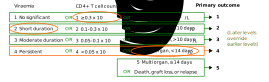
\includegraphics[width=7in]{parallel_composition_bandicoot.pdf}
  % \includegraphics[width=1in]{passport_ordinal_outcome_colorbar.png}
  \caption{\textbf{Parallel composition illustrated with the BANDICOOT outcome}.
    Ordinal outcome used in the planned BANDICOOT adaptive platform trial
    \citep{walkerCodesigningNovelOrdinal2025}. Illustrates \textbf{parallel
  composition} of component outcomes.} \label{fig:parallel_bandicoot}
\end{figure}

\subsubsection{Parallel composition by combining numeric scores}

One option: convert each input factor to a numeric value then sum them up.

A specific example of this, described e.g. by \citet{ongUnlockingDOORHow2023} in
the infectious disease context, is counting events of a particular
type (corresponds to converting the presence/absence of the event to
a 1/0 binary variable).

This doesn't respect the ordinal nature of the variables. That is, it
implicitly uses information about the \emph{differences} between levels.

\subsection{Pairwise comparison methods (win and DOOR) implicitly construct
ordinal outcomes}

Terms to define/distinguish:
\begin{itemize}
  \item Desirability of Outcome Ranking (outcome)
  \item Hierarchical composite endpoint (outcome)
  \item Prioritized outcomes (outcome)
  \item Win methods (win probability, win odds, win ratio) (effect
    measure; estimation methods)
  \item Generalized pairwise comparisons (effect measure)
\end{itemize}

These approaches implicitly \textbf{bundle together three different things}:
\begin{enumerate}
  \item Constructing an implicit ordinal outcome through
    hierarchical composition (complete tie-breaking/prioritized outcomes)
  \item
    Targeting a nonparametric effect measure defined via the
    ``pairs'' device (win
    probability/win ratio/win odds/etc.)
  \item Estimating that effect measure in a
    nonparametric/flexible manner using pairs, often also with devices for
    accounting for censoring
\end{enumerate}

This paper is focused on the first of these steps only.

Why is it useful to consider the three steps separately?

Consider some of the critiques of win methods in
\citet[e.g.~][]{ajufoFallaciesUsingWin2023}

\begin{itemize}
  \item Situating methods in their proper context can help
    trialists make informed choices among them
  \item Win methods can make use of
    plots and diagnostics for general ordinal outcomes, for the \emph{implicit}
    ordinal variable
    \begin{itemize}
      \item comparative CDF or ``survival''
        (complementary CDF) plots for assessing stochastic
        monotonicity \todo{this
          seems not done routinely? perhaps because of the difficulty
        of incorporating censoring?}
      \item ridit plots
        \citep{brossHowUseRidit1958,jansenRiditAnalysisReview1984} relative to a
        reference group, which should allow one to display both full
        eCDF information
        and also win statistics (based on the interpretation of the
          mean ridit as a win
        probability)
    \end{itemize}e.g.
  \item Ordinal regression models can use win
    methods for model checking; it is also possible to present a model-based win
    effect measure alongside a common odds ratio for example. See
    \citep{agrestiOrdinalProbabilityEffect2017} for example, which covers both
    latent variable and predicted probability versions.
  \item The outcomes
    \emph{implicitly} constructed using DOOR and win methods may contain many
    levels, and may contain levels where an effect is not so meaningful (e.g.
    time-to-death when the followup time is short). By \emph{explicitly}
    constructing the associated ordinal outcome one might be forced to be more
    aware of this
  \item What is a reasonable win analysis of a specific component
    score? From the traditional ordinal endpoint school of thought
    what would make
    most sense is to \emph{only tie-break for the lowest and highest
      levels of that
    score}, and e.g. plot eCDFs of this new variable. Is this what the plots do
    that break down wins and losses by component score?
\end{itemize}

Disadvantages of generalized pairwise comparison approaches
\begin{itemize}
  \item Inherited from downsides of complete tiebreaking
  \item Inherited from downsides of nonparametric/pairwise effect measures
  \item Regression methods exist, but are newer and less battle-tested
\end{itemize}

\section{Reasons to coarsen ordinal outcomes}

\subsection{Coarsening to avoid comparing ambiguous levels (validity)}

In the PASSPORT outcome (Figure \ref{fig:passport_outcome}), for
example, we include both digit
amputation and ECMO
any time within 28 days post-enrollment under the heading of
``adverse clinical events''.

Including these outcomes within the same level of an
ordinal outcome does not mean assuming that the two outcomes have the
\emph{same} utility. Rather it represents \emph{avoiding comparing}
their utilities. (This was something clinicians asked about more than once.)

Also, we "chunk" longer hospital stays more aggressively to avoid
small categories, for interpretability's sake.

\subsection{Coarsening for ease of communication}

Too many levels can make it hard to directly compare meaningful
proportions/probabilities.

(Outocmes with very many levels -- even up to of the order of 100 --
aren't really a problem for model fitting with modern software.)

Coarsening, including combining levels and replacing complete
tie-breaks with overrides, could help with this.

\section{Conclusions}

\newpage

\printbibliography

\end{document}
